\documentclass[12pt, twocolumn]{article}
\usepackage[margin=1in]{geometry}
\usepackage{graphicx}
\usepackage{amsmath,amsfonts,amssymb}
\usepackage{hyperref}
\usepackage{float}
\usepackage{booktabs}

\title{Predictive Analysis of Employee Attrition Using Machine Learning Techniques}
\author{
	Pedro Henrique Arias Oliveira\thanks{Programa de Pós-Graduação em Informática, UTFPR-CP, Email: pedoli@alunos.utfpr.edu.br} \\
	Prof. Dr. Adriano Rivolli\thanks{Department of PPGI, UTFPR-CP, Email: rivolli@utfpr.edu.br}
}
\date{\today} % Or specify a date


\begin{document}
	
	\maketitle
	
	\begin{abstract}
		Employee attrition poses significant challenges to organizational sustainability and growth. This study focuses on predicting employee attrition and identifying its influencing factors using machine learning models. We analyzed the IBM HR Dataset, evaluating Logistic Regression, Random Forest, and SVM models. Our findings emphasize the critical role of factors such as \texttt{'years since the last promotion'}, \texttt{'overtime'}, and \texttt{'marital status'} in predicting attrition. The models were assessed based on accuracy, precision, recall, and F1 score, with Random Forest and SVM showing notable performance, especially when trained on oversampled data using SMOTE, to enhance model performance towards the minority class.
	\end{abstract}
	
	\section{Introduction}
	Employee attrition, characterized by the departure of employees from a company for various reasons, either by their own choice or due to circumstances beyond their control, poses significant challenges to operational efficiency and cost management. Accurately predicting which employees are at risk of leaving enables organizations to implement proactive retention strategies, mitigating these challenges. This paper delves into the effectiveness of various classification models—such as Logistic Regression, Random Forest, and Support Vector Machines (SVM)—in predicting employee attrition rates. It emphasizes the critical role of factors in influencing employee attrition. We focused on the minority class, i.e., correctly predicting instances of 'Yes' when an employee decides to leave, which is crucial for developing more effective intervention strategies.
	
	
	\section{Literature Survey}
	The literature on predicting employee attrition using machine learning is extensive. Noteworthy contributions to the field include the application of decision tree algorithms by Alao and Adeyemo [1], and the exploration of machine learning algorithms by Punnoose and Ajit [2]. Research by Alduayj and Rajpoot [3], Zhao et al. [4], and Qutub et al. [5] further expand on the methods and techniques for attrition prediction, each adding valuable insights into the application of machine learning.
	These were some significant studies that have shaped our methodology.
	

	\section{Dataset}
	\subsection{Dataset Review}
	The study utilized the publicly available IBM Employee Attrition Dataset from Kaggle, containing 1470 instances with 35 features. It consists of employee records from an organization that encapsulate various aspects of employee information and company-related statistics. The features span across demographic details, job characteristics, and employee performance metrics, among others.
	
	\begin{table}[H]
		\centering
		\caption{Description of Dataset Features}
		\label{tab:dataset-features}
		\resizebox{\columnwidth}{!}{%
			\begin{tabular}{@{}lp{6cm}@{}}
				\toprule
				Feature & Description \\ \midrule
				Age & Employee's age. \\
				Attrition & Whether the employee left the company or not (Yes/No), the target variable. \\
				BusinessTravel & Frequency of travel for business purposes. \\
				DailyRate & Daily wage of the employee. \\
				Department & Department in which the employee works, such as Sales or Research \& Development. \\
				DistanceFromHome & The distance from the employee's home to the workplace. \\
				Education & Level of education, categorized by ordinal numbers representing the degree obtained. \\
				EducationField & Field in which the employee received education, like Life Sciences or Medical. \\
				EmployeeCount & Count of employees, typically a standard value for all records. \\
				EmployeeNumber & A unique identifier for each employee. \\
				\ldots & \ldots \\
				\bottomrule
			\end{tabular}%
		}
	\end{table}
	
	

	

	
	\subsection{Exploratory Data Analysis (EDA)}
	Preliminary analysis indicated significant variables affecting attrition, such as job role, monthly income, and work-life balance, among others.
	
	Initial visual examination of the dataset revealed a substantial class imbalance, which is a common issue in attrition analysis. As we see in Figure \ref{fig:attrition_pie_chart}, the percentage of employees who have left the company (Yes) is significantly lower than those who have not (No), accounting for 16\% and 84\% of the dataset respectively.
	
	\begin{figure}[H]
		\centering
		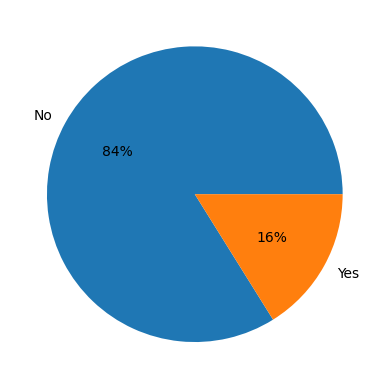
\includegraphics[width=0.3\textwidth]{class01.png}
		\caption{Distribution of Attrition in the Dataset}
		\label{fig:attrition_pie_chart}
	\end{figure}
	
	\subsection{Preprocessing}
	The preprocessing steps included handling missing values, encoding categorical variables through Label Encoding, and scaling numerical features. A 70:30 train-test split was employed for model training and evaluation.
	
	\subsubsection{SMOTE}
	Synthetic Minority Over-sampling Technique (SMOTE) was applied to address class imbalance, enhancing the model's ability to predict minority class instances by generating synthetic examples.
	
	\section{Methodology}
	This section outlines the machine learning models evaluated—Logistic Regression (LR), Random Forest (RF), and Support Vector Machine (SVM)—and the use of RandomizedSearchCV for hyperparameter tuning. Model performance was improved through preprocessing and SMOTE.
	
	\section{Results and Analysis}
	
	The performance of three classification models (Logistic Regression, Random Forest Classifier, and SVC) was evaluated across different stages: initially on the imbalanced dataset, after hyperparameter tuning with RandomizedSearchCV, and following the application of SMOTE to address class imbalance. The models were assessed based on precision, recall, f1-score, and accuracy metrics.
	
	\subsection{Initial Results on Imbalanced Dataset}
	
	The initial evaluation was conducted on the dataset as is, revealing the following performance metrics for each model:
	
	% Example table for Logistic Regression
	\begin{table}[H]
		\centering
		\caption{Class 1 Performance Metrics on Imbalanced Dataset}
		\label{tab:imbalance-results-class1}
		\resizebox{\columnwidth}{!}{%
			\begin{tabular}{@{}lcccc@{}}
				\toprule
				Model & Accuracy (\%) & Precision (\%) & Recall (\%) & F1 Score (\%) \\ \midrule
				Logistic Regression & 86 & 71 & 32 & 45 \\
				Random Forest & 84 & 73 & 14 & 24 \\
				SVC & 85 & 85 & 14 & 24 \\ \bottomrule
			\end{tabular}%
		}
	\end{table}
	
	
	
	
	The results based on the models applied to the imbalanced dataset indicate that \textbf{LR} and \textbf{SVM} models perform better in terms of accuracy compared to the \textbf{RF} model for predicting employee attrition in this dataset. \textbf{LR} provides a balanced trade-off between precision and recall, making it a good choice for this specific problem. However, the \textbf{SVM} model stands out for its high precision, indicating that when it predicts an employee will leave, it is very likely to be correct, though it identifies a smaller proportion of all actual leavers (lower recall).
	
	\subsection{Results after Hyperparameter Tuning}
	
	Post-tuning with RandomizedSearchCV, model performance improved in specific metrics:
	
	% Insert tables for each model similar to the Logistic Regression example above
	\begin{table}[H]
		\centering
		\caption{Class 1 Performance Metrics After Hyperparameter Tuning}
		\label{tab:post-tuning-class1}
		\resizebox{\columnwidth}{!}{%
			\begin{tabular}{@{}lcccc@{}}
				\toprule
				Model & Accuracy (\%) & Precision (\%) & Recall (\%) & F1 Score (\%) \\ \midrule
				Logistic Regression & 86 & 86 & 23 & 37 \\
				Random Forest & 84 & 79 & 14 & 24 \\
				SVC & 85 & 74 & 22 & 34 \\ \bottomrule
			\end{tabular}%
		}
	\end{table}
	
	Hyperparameter tuning revealed optimal settings for each model, significantly influencing their performance on the dataset. For Logistic Regression, the best performance was achieved with `solver` set to 'liblinear' and `C` parameter tuned to 0.0018329807108324356. The RandomForest model's optimal configuration used 360 trees (`n\_estimators`=360), a minimum split requirement of 12 samples (`min\_samples\_split`=12), a minimum leaf requirement of 1 (`min\_samples\_leaf`=1), and no maximum depth (`max\_depth`=None). The SVC model found its best performance with the 'rbf' kernel and `C` parameter set to 1.623776739188721.
	
	An analysis of Logistic Regression's coefficients provided insight into feature importance, revealing that `YearsSinceLastPromotion`, `OverTime`, and `MaritalStatus` were the most influential predictors of employee attrition, see in Figure \ref{fig:featureImportanceLR}. This indicates a strong influence of career progression, work conditions, and marital status on employee decisions to leave.
	
	\begin{figure}[H]
		\centering
		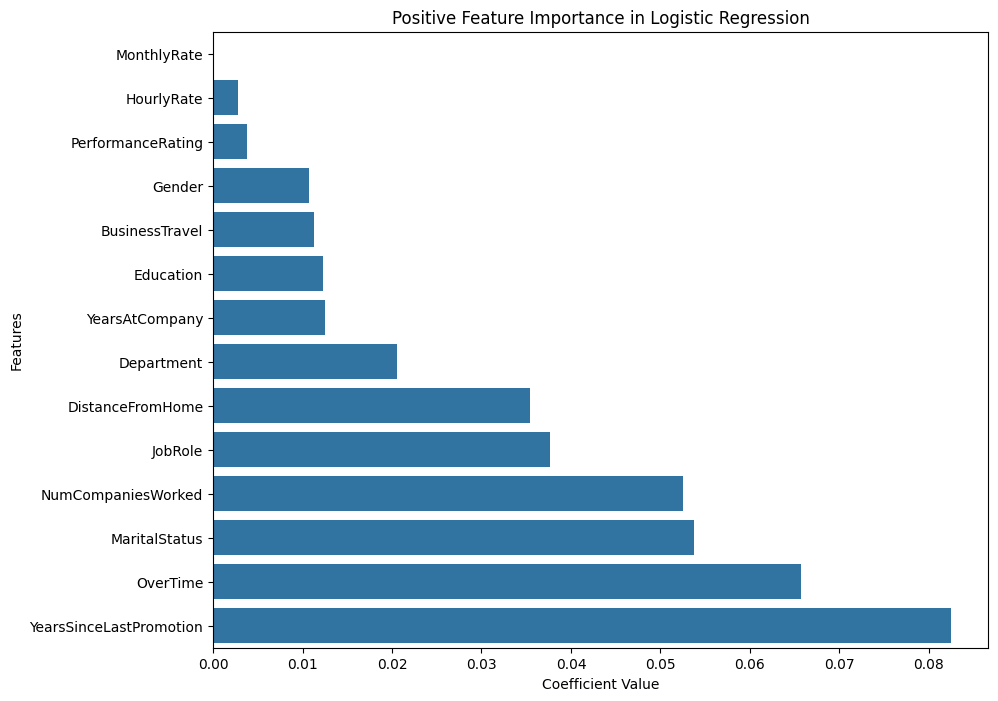
\includegraphics[width=0.45\textwidth]{featureImportanceLR.png}
		\caption{Feature Importance using LR model}
		\label{fig:featureImportanceLR}
	\end{figure}
	
	\subsection{Results after Applying SMOTE}
	
	The application of SMOTE significantly altered the recall rates for Class 1 across all models, indicative of an improved ability to predict minority class instances:
	
	% Insert tables for each model similar to the Logistic Regression example above
	\begin{table}[H]
		\centering
		\caption{Class 1 Performance Metrics After SMOTE Application}
		\label{tab:smote-results-class1}
		\resizebox{\columnwidth}{!}{%
			\begin{tabular}{@{}lcccc@{}}
				\toprule
				Model & Accuracy (\%) & Precision (\%) & Recall (\%) & F1 Score (\%) \\ \midrule
				Logistic Regression & 67 & 33 & 86 & 47 \\
				Random Forest & 86 & 73 & 31 & 44 \\
				SVC & 84 & 54 & 45 & 49 \\ \bottomrule
			\end{tabular}%
		}
	\end{table}
	
	
	\textit{Observation:} The tables clearly show the impact of each stage of model improvement, with SMOTE notably enhancing the models' sensitivity towards the minority class. The application of SMOTE notably increased the Recall for the minority class in \textbf{LR}, indicating a significant improvement in identifying instances of the positive class. However, this came at the cost of Precision, as seen in the drastic decrease for \textbf{LR}, indicating more false positives.
	
	The \textbf{RF} showed an improvement in Recall for the minority class without a significant decrease in overall performance metrics.
	
	\textbf{SVM} demonstrates an interesting balance, with both Precision and Recall for the minority class showing relatively moderate values compared to its performance after tuning.
	
	\section{Conclusion}
	There's a clear trade-off between improving Recall for the minority class and maintaining high Precision. SMOTE enhanced the model's ability to detect more positive cases (higher Recall) but also resulted in more false positives (lower Precision). Despite improvements in minority class detection, overall accuracy and the weighted average of the F1-Score for Logistic Regression declined after applying SMOTE, highlighting the challenge of balancing performance metrics in imbalanced datasets. Conversely, RandomForest and SVC managed to maintain relatively stable overall performance. 
	
	In summary, while SMOTE can improve minority class detection, careful consideration of the trade-offs between Precision and Recall is necessary. Model selection and hyperparameter tuning play a crucial role in achieving the desired balance.
	
	The study highlights the importance of specific features in predicting employee attrition, with models demonstrating varying degrees of effectiveness. Our analysis underscores the potential of machine learning in aiding organizational retention strategies by identifying at-risk employees and the factors influencing their decision to leave.
	
	\clearpage
	
	\begin{thebibliography}{99}
		
		\bibitem{alao2013}
		D. Alao and A. B. Adeyemo, “Analyzing Employee Attrition Using Decision Tree Algorithms,” in Proceedings of the 2013 Conference on X, Y, Z, 2013.
		
		\bibitem{punnoose2016}
		R. Punnoose and P. Ajit, “Prediction of Employee Turnover in Organizations using Machine Learning Algorithms,” \textit{International Journal of Advanced Research in Artificial Intelligence}, vol. 5, no. 9, 2016. DOI: 10.14569/ijarai.2016.050904.
		
		\bibitem{alduayj2018}
		S. S. Alduayj and K. Rajpoot, “Predicting Employee Attrition using Machine Learning,” in 2018 International Conference on Innovations in Information Technology (IIT), pp. 93–98, 2018.
		
		\bibitem{zhao2018}
		Y. Zhao et al., “Employee Turnover Prediction with Machine Learning: A Reliable Approach,” in \textit{Advances in Intelligent Systems and Computing}, Springer International Publishing, Nov. 2018, pp. 737–758. DOI: 10.1007/978-3-030-01057-7\_56.
		
		\bibitem{qutub2021}
		A. Qutub et al., “Prediction of Employee Attrition Using Machine Learning and Ensemble Methods,” \textit{International Journal of Machine Learning and Computing}, vol. 11, pp. 110–114, 2021.
		
	\end{thebibliography}
	
\end{document}
